\section{Problemstellung} \label{Problemstellung}

Um eine formal korrekte Identitätskette aufzubauen, wird eine verlässliche Basis, grade auch dann, wenn Futtermittel- und Logistik-Informationen unter allen Marktteilnehmern ausgetauscht werden müssen, benötigt. Grundlage dafür ist die EU-Verordnung 178/02 (insbesondere Artikel 18 und 19), welche die Notwendigkeit beschreibt, dass jeder Akteur der Lieferkette dafür verantwortlich ist, nachzuweisen von wem er seine Waren bezogen und an wen er seine Waren geliefert hat \citep{EPER2002}.

% Aktuelle Lösung beim Praxispartner erläutern und auf Probleme hinweisen!
Als konkretes Beispiel wird beim Praxispartner Westfleisch SCE mbH zur Realisierung einer Chargenrückverfolgung die Software \ac{gbt} vom Hersteller SAP eingesetzt. Mithilfe dieser Software werden die Stammdatenobjekte \textit{Charge}, \textit{Produkt} und \textit{Geschäftspartner} verwaltet und mit dem \ac{erp} System integriert. \ac{gbt} ist dabei als zentrales System konzipiert, welches über eine Schnittstelle von Akteuren der Lieferkette mit Informationen zu einer Charge beliefert werden kann. Diese Schnittstelle verwendet \textit{\acs{idoc}}\footnote{Ein \ac{idoc} ist ein Container für den Datenaustausch zwischen SAP und Nicht-SAP-Systemen \citep{SAP2019}.} bzw. \textit{\acs{xml}}\footnote{Die \ac{xml} ist eine Auszeichnungssprache zur Darstellung hierarchisch strukturierter Daten im Format einer Textdatei \citep{Yergeau2008}.} als Austauschformat. Der eigentliche Austausch erfolgt dabei entweder manuell über einen Dateiimport/-export Mechanismus oder über das Internet mittels des \textit{\acs{http}}\footnote{\ac{http}} Protokoll. Bei diesem Austausch besteht grundsätzlich die Möglichkeit, dass Datensätze vor dem Austausch oder nachträglich verändert werden können - ohne das Teilnehmer der Lieferkette hiervon etwas mitbekommen würden.

Der Einsatz von \textit{Blockchain-Technologie} könnte in dieser Situation eine Lösung darstellen. Eine \textit{Blockchain} ist ein dezentrales System zur manipulationssicheren Speicherung von Informationen in sog. \textit{Blöcken} die untereinander durch kryptographische Methoden verkettet sind - daher auch der Name \textit{Blockchain}. Eine \textit{Blockchain} verwendet verschiedenste Verfahren zur Konsensbildung innerhalb des Netzwerks, um sicherzustellen das neue \textit{Blöcke} und die darin enthaltenen Transaktionen vom gesamten Netzwerk validiert und verifizert werden bevor der \textit{Block} in die \textit{Blockchain} geschrieben wird \citep[siehe auch][]{Nakamoto2009, Buterin2014, Cardano2017, carVertical}.

Außerdem kann eine \textit{Blockchain} durch den Einsatz einer kryptographischen \textit{Hashfunktion}\footnote{Spezielle Form einer Hashfunktion, welche kollisionsresistent ist. Es ist praktisch nicht möglich, zwei unterschiedliche Eingabewerte zu finden, die einen identischen Hashwert ergeben \citep{Menezes1997}.} zur Bildung einer Prüfsumme für jeden \textit{Block} innerhalb der \textit{Blockchain} sicherstellen, dass bereits persistierte Informationen nicht ohne weiteres manipuliert werden können. Im Idealfall ist eine \textit{Blockchain} dezentral konzipiert, was bedeutet, das jeder Teilnehmer eines \textit{Blockchain} Netzwerks eine exakte Kopie des Datenbestands lokal vorhält. Hierdurch soll sichergestellt werden, das auch bei einem Ausfall oder einer Kompromittierung einzelner Teilnehmer das Gesamtsystem weiterhin in seiner Funktion stabil bleibt \citep{Drescher2017, Tribis2018}.

% Bitcoin war die erste Generation von Blockchain. Die Bitcoin \textit{Blockchain} ist in der Lage Einheiten der Bitcoin Währung zwischen zwei Parteien zu versenden ohne das eine Bank oder eine Clearingstelle diese Transaktion validieren muss. \citep{Nakamoto2009} Ethereum war die zweite Generation einer Blockchain. Im Vergleich zur Bitcoin \textit{Blockchain} lassen sich mit dem Ethereum Netzwerk auch sog. \ac{sc} erstellen und ausführen.\citep{Buterin2014} Skalierbarkeit und Interoperabilität spielen in dieser Generation eine der entscheidenden Rollen. \citep{Cardano} \textit{Blockchain} Anwendungen im Enterprise Bereich exisiteren maximal auf dem Reißbrett.\\

% Die Kernidee hinter der Blockchain-Technologie ist es einen Intermediär zu substituieren, der nur eingesetzt wurde um eine neutrale Vertrauensbildung zu ermöglichen. \ac{dlt} verfolgt dabei den Ansatz die Vertrauensbildung, den Ablauf von Transaktionen und deren sichere Festschreibung mit mathematischen und kryptographischen Methoden zu realisieren. Im Kontrast zum konventionellen Intermediär, welcher durch eine dritte Person oder Institution wie z.B. eine Bank oder einen Notar repräsentiert wird.\\

% Für das Problem der Einigkeit über den Zustand eines Werts innerhalb der \textit{Blockchain} sind zwei generelle Verfahren etabliert. Die \ac{pow} und \ac{pos} genannten Algorithmen nutzen unterschiedliche Ansätze um Konsens innerhalb eines Netzwerks zu bilden und so Vertrauen herzustellen. Beide Verfahren haben ihre Vor- und Nachteile.\\

% Prozesse die einen transaktionalen Charakter besitzen und oft auch ein oder mehrere Vermittlerstellen zwischengeschaltet haben würden sich Ideal für den Einsatz von \textit{Blockchain-Technologie} eignen. Fehlende Standards und generelle Unsicherheit verhindern allerdings den flächendeckenden Einsatz der Technologie.\\

% Abbildung \ref{fig:statista-huerden-blockchain-2016} zeigt die Ergebnisse einer Umfrage des Fachmagazins Cofinpro zum Thema \glqq Wo sehen Sie Hürden für die Blockchain-Technologie?\grqq~. So scheinen die mit Abstand größten Einstiegsbarrieren fehlende Standards und rechtliche Regelungen zu sein.

% \begin{figure}[h!]
% 	\centering
% 	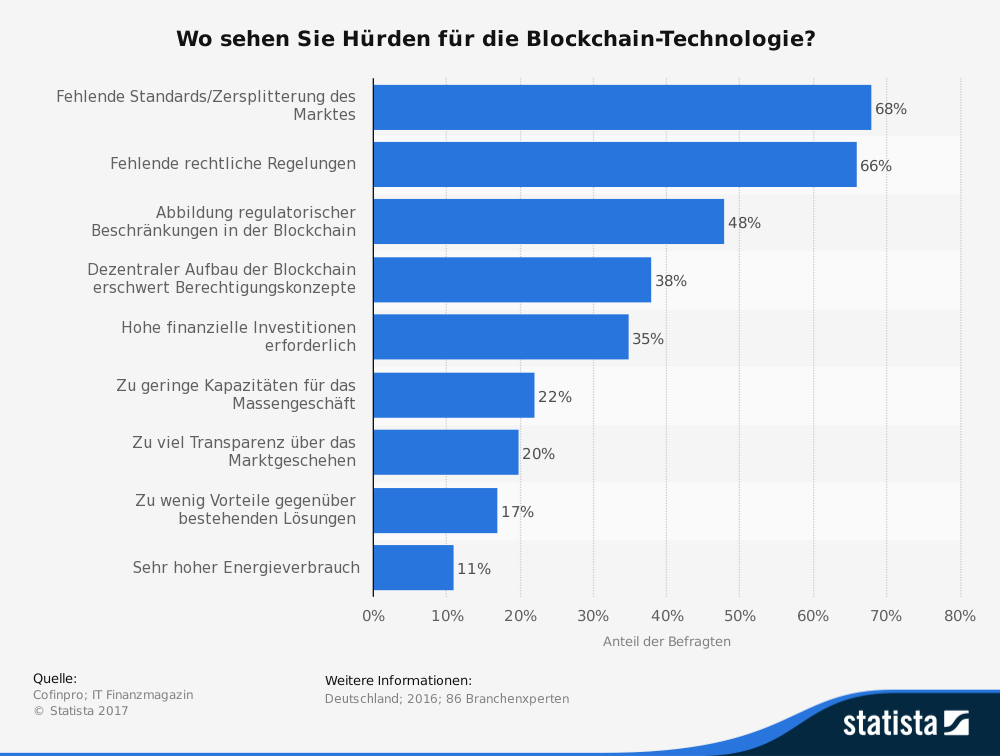
\includegraphics[width=0.7\linewidth]{pictures/Statista-Huerden-Blockchain-2016}
% 	\caption[Statista \textit{Blockchain} Umfrage]{Cofinpro - Wo sehen Sie Hürden für die \textit{Blockchain-Technologie}? \citep{Cofinpro}}
% 	\label{fig:statista-huerden-blockchain-2016}
% \end{figure}

Aus den beschriebenen Sachverhalten ergibt sich für eine zeitnahe und transparente Rückverfolgung von Chargen über den gesamten Verlauf der Wertschöpfungskette in Produktionsnetzwerken mittels \textit{Blockchain-Technologie} folgende Forschungsfrage:

\begin{itemize}
  \item[\textbf{FF1}] \textbf{Wie kann die Rückverfolgbarkeit von Chargen in der Fleischwarenindustrie entlang der gesamten Lieferkette mithilfe von Blockchain-Technologie realisiert werden?}
  \begin{itemize}
    \item[FF1.1] Welche Anforderungen an ein System zur Rückverfolgbarkeit von Chargen werden seitens der Fleischwarenindustrie gestellt?
    \item[FF1.2] Welche Daten müssen in einer \textit{Blockchain} persistiert werden, um eine Rückverfolgbarkeit zu ermöglichen?
    \item[FF1.3] Welche \textit{Blockchain-Technologie} kommt in Frage um FF1 zu realisieren und den spezifischen Anforderungen der Fleischwarenindustrie gerecht zu werden?
    \item[FF1.4] Welche Systemarchitektur erfüllt die Anforderungen der Fleischwarenindustrie, um eine Chargenrückverfolgung zu realisieren?
    % \item[FF1.4] Wie könnte eine Systemarchitektur für ein durch \textit{Blockchain-Technologie} gestütztes System konzipiert sein?
  \end{itemize}
\end{itemize}

% \begin{figure}[h!]
% 	\centering
% 	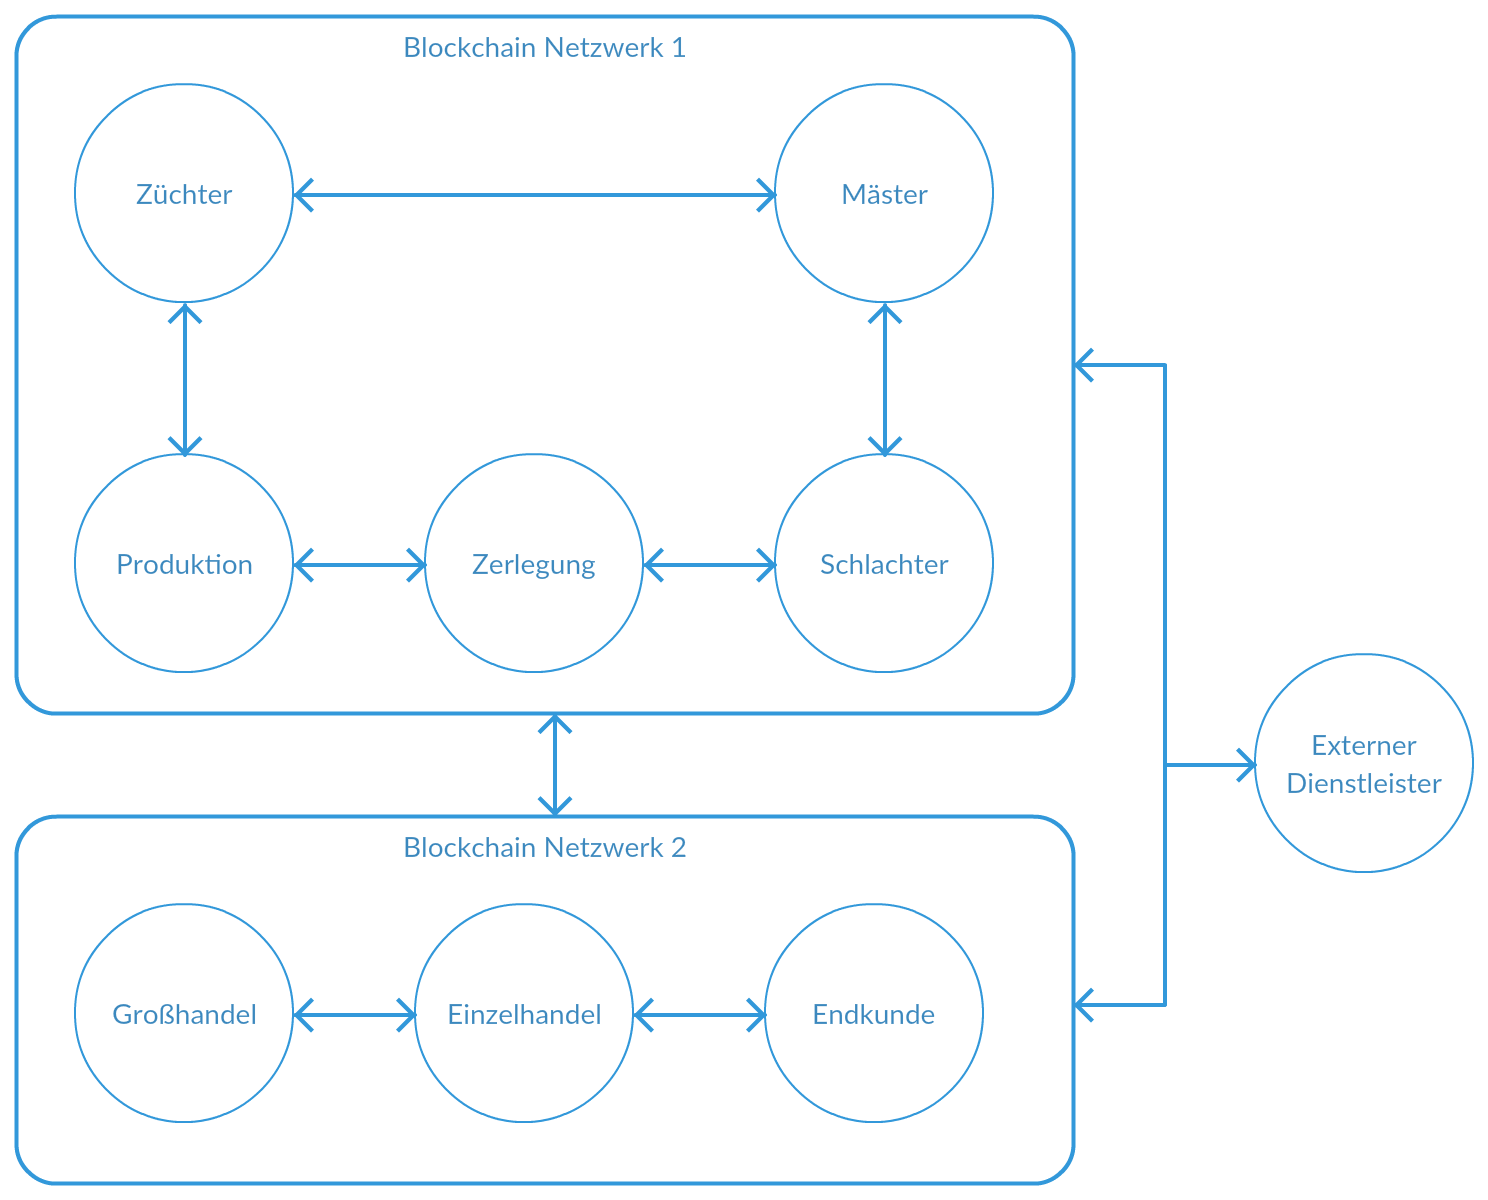
\includegraphics[width=0.8\linewidth]{pictures/Multi-Blockchain-Example}
% 	\caption[Multiple Blockchains innerhalb der Lieferkette]{Multiple Blockchains innerhalb der Lieferkette (eigene Darstellung)}
% 	\label{fig:multi-blockchain-example}
% \end{figure}

\newpage
